\documentclass{IEEEtran}

\usepackage{graphicx}
\usepackage{color}
\usepackage{colortbl} % for \rowcolor
\usepackage{caption}
\usepackage{subcaption}
\usepackage[bookmarks=false]{hyperref}
\usepackage{algpseudocode}
\usepackage{algorithm}
\algnewcommand\algorithmicforeach{\textbf{for each}}
\algdef{S}[FOR]{ForEach}[1]{\algorithmicforeach\ #1\ \algorithmicdo}

\newcommand{\todo}[1]{\marginpar{\parbox{18mm}{\flushleft\tiny\color{red}\textbf{TODO}:
      #1}}}
\definecolor{headcolor}{gray}{0.9}


\begin{document}

\title{Performance Evaluation of Big Data Processing Strategies for Neuroimaging}

\author{
  \IEEEauthorblockN{
    Val\'erie Hayot-Sasson and 
    Tristan Glatard
  }\\
  \IEEEauthorblockA{
    Department of Computer Science and Software Engineering, Concordia University, Montreal, Qu\'ebec, Canada
  }
}

\maketitle

\begin{abstract}
  
\end{abstract}

% Talk about containers somewhere?

\section{Introduction} % 1 page with abstract

Big Data processing engines reduce data-related overheads, through 
use of concepts such as data locality, in-memory computing, and lazy evaluation.
Data locality-aware scheduling, popularized by the MapReduce~\cite{dean2008mapreduce} 
framework, runs tasks to the nodes holding the data rather than 
performing costly data transfers across the network. In-memory 
computing, adopted by MapReduce's successor Apache 
Spark~\cite{zaharia2016apache}, caches data in memory whenever 
possible, reducing costly disk I/Os between pipeline steps. 
Lazy evaluation, also used in Spark, means that results are computed only 
when necessary, enabling further performance optimizations. Frameworks 
such as
MapReduce and Spark have become mainstream tools for data analytics, 
although many others, such as 
Dask~\cite{rocklin2015dask}, are emerging. 
Meanwhile, several scientific 
domains including bioinformatics, physics or astronomy, have entered 
the Big Data era due to increasing data volumes and variety. 
However, the adoption of Big Data engines for scientific data analysis 
remains limited, perhaps due to the widespread availability of 
scientific processing engines such as Pegasus~\cite{deelman2005pegasus} or
Taverna~\cite{oinn2004taverna}, and the adaptations required in Big 
Data processing engines for scientific computing. 

Scientific applications differ from the typical Big Data use 
cases, which might explain the remaining gap between Big Data and 
scientific engines. \todo{This sentence is extremely long} While Big Data applications mostly target text 
processing (e.g. Web search, frequent pattern mining, recommender 
systems~\cite{leskovec2014mining}), implemented in consistent software 
libraries and running on clouds or dedicated commodity clusters with 
locality-aware file systems such as the Hadoop Distributed File System 
(HDFS~\cite{shvachko2010hadoop}), scientific applications often involve 
binary data such as images and signals, processed by command-line tools 
using a mix of programming languages (C, Fortran, Python, shell 
scripts), and are deployed on large, shared clusters where 
data is fetched from data nodes to compute nodes using centralized shared file 
systems such as Lustre~\cite{schwan2003lustre}. Such differences in 
applications and infrastructures have important consequences. To 
mention only one, in-memory computing requires instrumentation to be 
applied to command-line tools. Moreover, performance is only one of the important
aspects to scientific computing. Other important aspects include reproducibility 
and provenance tracking. While these are minimally addressed by Big Data
processing engines, it is currently insufficient for scientific computing. 
Incorporation of provenance techniques into frameworks such are Spark are
currently being investigated~\cite{samba}.

Technological advances of the past decade, in particular page caching 
in the Linux kernel~\cite{love2010linux}, in-memory file systems 
(tmpfs) and memory-mapped files\todo{check that} might also 
explain the lack of adoption of Big Data engines for scientific 
applications.
In-memory computing would then be a feature provided by 
the operating system rather than by the engine itself. The frontier 
between these two components is blurred and needs to be clarified.


% https://ntrs.nasa.gov/archive/nasa/casi.ntrs.nasa.gov/20130001600.pdf

Neuroimaging, our primary field of interest, is no exception to the 
generalized rise of data volumes in science, due to the joint increase 
of image resolution and subject cohort sizes~\cite{van2014human}. 
Processing engines have been developed with neuroinformatics 
applications in mind, for instance Nipype~\cite{gorgolewski2011nipype} 
or the Pipeline System for Octave and Matlab 
(PSOM~\cite{bellec2012pipeline}). Big Data engines have been used for 
neuroimaging applications too, including in the Thunder 
project~\cite{freeman2014mapping} and in more specific works such 
as~\cite{makkie2019fast}. However, no quantitative performance 
evaluation has been conducted on neuroimaging applications to assess the 
added-value of Big Data engines compared to traditional processing engines.

This paper addresses the following questions:
\begin{enumerate}
\item What is the effect of in-memory computing, lazy evaluation and data locality on current neuroimaging applications?
\item Can in-memory computing be effectively enabled by the operating system rather than the data processing engine?
\end{enumerate}

Answers to these questions have important implications. 
In~\cite{mehta2017comparative}, a comparative study of Dask, Spark, 
TensorFlow, MyriaDB, and SciDB on neuroinformatics use-cases is 
presented. It concludes that these systems need to be extended to 
better address scientific code integration, data partitioning, data 
formats and system tuning. We argue 
that such efforts should only be conducted if substantial performance 
improvements are expected from in-memory computing, lazy 
evaluation\todo{are we talking about lazy evaluation at all?} or data 
locality. On the other hand, neuroimaging data processing engines are 
still being developed, and it is legitimate to wonder whether these 
projects should just be migrated to Spark, Dask, or other Big Data 
engines.

Our study focuses on performance. We intentionally do not intend to 
compare Big Data and scientific data processing engines on the grounds 
of workflow language expressivity, fault-tolerance, provenance capture and 
representation, portability or reproducibility, which are otherwise 
critical concerns. Besides, our study of performance focuses on the 
impact of data writes and transfers. It purposely leaves out task 
scheduling to computing resources, to focus on the understanding of 
data writes and movement. Task scheduling will be part of our 
discussion though.

Infrastructure-wise, we focus on the case of High-Performance Computing 
(HPC) clusters that are typically available through University 
facilities or national computing infrastructures such as XSEDE, Compute 
Canada or DEISA \todo{add links}, as this is the type of platform which 
is typically available to neuroscientists. We assume that HPC systems 
are multi-tenant, that compute nodes are accessible through a batch 
scheduler, and that a file system shared among the compute nodes is 
available, for instance Lustre. We intentionally leave distributed, 
HDFS-like file system out, as initiatives to deploy them in HPC 
centers, for instance Hadoop on-demand~\cite{hadoop-on-demand} have not 
become mainstream yet.


\todo{Perhaps talk about modeling and simulation here.}

Our methods, including performance models, processing engines, \todo{Make this paragraph more informative}
applications and infrastructure used are described in 
Section~\ref{sec:methods}. Section~\ref{sec:results} presents our 
results which we discuss in Section~\ref{sec:discussion}. 
Section~\ref{sec:conclusion} concludes on the answer to our two research questions.

\section{Materials and Methods} % 4 pages
\label{sec:methods}

\todo{Maybe add an intro to this section, to outline it}

\subsection{Engines} % 1.5 pages

\subsubsection{Apache Spark}

Apache Spark is a popular Scala-based processing framework for Big Data, with
APIs in Java, Python and R. Its 
generalized nature allows Spark to not only be applied to batch workflows,
but also SQL queries, iterative machine learning applications, 
data streaming and graph processing. Spark's
main features include data-locality, in-memory processing and lazy evaluation,
which it achieves through its principle abstraction, the Resilient Distributed 
Dataset (RDD). 

An RDD is an immutable parallel data structure that achieve fault-tolerance 
through the concept of lineage~\cite{zaharia2010spark}. Rather than permitting
fine-grained transformations, only coarse-grained transformations (applying to
many elements in the RDD), can be applied, thereby making it simple to keep a 
log of how the data was modified. This log, known as the lineage, is used
to reproduce any lost data.

Two types of operations can be performed on RDDs:
transformations and actions. Applying a transformation to an RDD produces a new,
child, RDD through a narrow or wide dependency. A narrow dependency signifies 
that the child is only dependent on a single parent partition, whereas a child 
RDD is dependent on all parent partitions in a wide dependency. Examples of 
Spark transformations include map, filter and join. To materialize an RDD, an
action must be performed, such as a reduce or a collect.

All actions and wide dependencies require a shuffle -- Spark's most costly
operation. Every shuffle begins with each map task saving its data to local
files to be fetched by the shuffle operation. The shuffle operation then 
redistributes the data across the partitions as requested. A shuffle marks a 
stage boundary in Spark. In other words, a shuffle will not begin until all 
dependent map tasks \todo{shouldn't it be 'actions'?} have completed.

Spark will spill RDD data to disk whenever the complete dataset does not fit in
memory. Moreover, as Spark transformations generate new RDDs and numerous 
transformations may occur in a single application, Spark implements a Least-Recently Used (LRU) eviction
policy. If an evicted RDD needs to be reused, Spark will recompute it using the
lineage data collected. It therefore becomes of great importance to persist to
memory and/or 
disk RDDs which will be reused throughout the application, particularly if the
recomputation is costly. 
%mention results in thunder paper

Data locality in Spark is achieved through the  scheduling of task to partitions which have the
data loaded in memory. If the data is instead stored on HDFS, the scheduler will
assign it to one of the preferred locations specified by HDFS. Spark's scheduler
utilizes delay scheduling to optimize fairness and locality for all tasks.
%improve paragraph

Three different types of schedulers are compatible with Spark: 1) Spark 
Standalone, 2) YARN~\cite{vavilapalli2013apache} and 3) Mesos~\cite{hindman2011mesos}. The Spark Standalone
scheduler is the default scheduler. YARN was a scheduler designed for Hadoop~\cite{white2012hadoop}
clusters. It is prepackaged with Hadoop installations. In contrast to YARN, 
Mesos was designed to be used in multitenant cluster environments. In our experiments,
we focus on the Spark Standalone cluster.

Executing Spark applications on HPC systems with Spark-unaware schedulers may
be inefficient. The amount of resources requested by Spark may impede Spark-cluster
scheduling time. Using pilot-scheduling strategies to add nodes to the Spark cluster
as they are allocated by the underlying schedulers may speedup allocation and 
overall processing time. This, however, is not studied in the current paper.

As Spark is frequently used by the scientific community, we designed our 
experiments using the PySpark API. This is at a cost to performance as the PySpark
code must undergo Python to Java serialization.


%% Main concepts
% pipeline description
% detailed description relevant to the experiment
% how shuffle works
% how data locality is implemented
% spills to disk when dataset (and derived data) is too large for memory
% Lazy evaluation
% persistence (refer to Thunder)
% multiple schedulers: we focus on Spark Standalone
% overlay cluster: not considered here as this would be scheduling

%% Technical details
% data serialization to Java (we use Python as most neuroinformatics do)
% limitation in size of RDD element, due to java implementation of binary data
% memory management: don't give too much memory to executors or GC
%  many places recommend limiting to 5 cores/executor, no one explains why
% more on tuning?

\subsubsection{Nipype}

Nipype is a popular Python neuroimaging processing engine. It aims at being a 
solution for easily creating reproducible neuroimaging workflows. Although Nipype
does not employ any Big Data processing strategies, it provides access to numerous
plugins to schedulers found in most clusters readily available to researchers, 
such as SGE, PBS, SLURM and HTCondor\todo{expand acronyms}. It also includes its own scheduler, MultiProc,
for parallel processing on single nodes. Nipype also includes many built-in 
interfaces to commonly used neuroimaging tools to be incorporated within the 
workflows. Nipype's ability to easily parallelize workflows in researcher-available 
cluster setups, capture detailed provenance information necessary for reproducibility,
and allow users to easily integrate existing neuroimaging tools, make it preferable
to existing Big Data solutions, which would necessitate modification to achieve this.

Jobs, or Interfaces, in Nipype, are encapsulated by a Node. A Node dictates that
the job will execute on a single input. However, the MapNode, 
a child variant of the Node, can execute on multiple inputs. All tasks in
Nipype execute in their own uniquely named subdirectory which facilitates the provenance 
tracking of inputs and outputs. This also enables checkpointing of the workflow.
In the case of Node failure or application modification, only the nodes who have
been modified (verified by hash) are re-executed.

In order for Nipype to operate as intended, a filesystem shared by all the nodes 
is required. However, it is still possible to save to a non-shared local filesystem, 
but it may come at the expense of fault-tolerance \todo{explain why}. Moreover, the user will need to
ensure that the files are appropriately directed to the nodes that require them as
there is no guarantee of data locality in Nipype.


% pipeline description: map nodes and their limitations
% general description relevant to the experiment
% two plugins
% provenance
% file system caching
% memory management (bad?)
% Nipype only has data locality becausae we use multiproc. Data locality is emulated by manual decisions on scheduling.

\subsection{Data Storage Locations}

Data storage location is critical to the performance of Big Data 
applications on HPC clusters.
Data may reside in the engine memory, on 
a file system whose content reside in virtual memory (for instance 
tmpfs), on disks local to the processing node, or on a shared 
file system. Table~\ref{table:features} summarizes the Big Data 
strategies that can be used depending on the data location. In 
addition, lazy evaluation is available in Spark regardless of data 
location. The remainder of this Section explains this Table and 
provides related performance models.
\begin{table}
\centering
\begin{tabular}{c|cc}
   \rowcolor{headcolor}
    Data Location                 & In-Memory     & Data Locality        \\
    \rowcolor{headcolor}
                                  & Computing     &                     \\
                                  \hline          
In-memory                         &   Y           & Y                       \\
tmpfs                             &   Y           & Y                   \\
Local Disk                        & Page Caching  & Y                   \\
Shared File System                & Page Caching  & N                
% data locality is somehow present in shared fs due to page caching again.
\end{tabular}
\caption{Big Data strategies on a shared HPC cluster.}
\label{table:features}
\end{table}

\subsubsection{In-Engine-Memory and In-Memory File System} 

 The main difference between storing the data in the engine memory, as in Spark, 
 and simply writing to an in-memory file system, such as tmpfs, is 
 related to what happens when the processed data fills up the available 
 memory. In case engine memory is used, the engine has to cleanup 
 unused data with some strategy to avoid crashes. In case an in-memory 
 file system is used, the kernel starts swapping memory to disk, and 
 the performance becomes that of local disk writes. In our experiments, 
 we will explore the region  when the data consumed by the 
 application approaches the threshold of available memory.

\subsubsection{Local Disk (Page Caching)} % 0.5 page



% Perhaps refer to this: https://ieeexplore.ieee.org/abstract/document/5496998

% measured disk bandwidth with random I/O, very different from sequential

Storing data on local disks obviously enables data locality as tasks 
executed on the node where their input files reside do not require to 
transfer input or output data. However, in absence of a more specific 
file system such as the Hadoop Distributed File System (HDFS) to handle 
file replication across computing nodes, data locality comes at the price
of stringent scheduling restrictions, as tasks can only be scheduled to the
single node that contains their input data.
% this brings data locality but not at the level of HDFS because replication isn't there and 
% there is only 1 single option to schedule a task while preserving data locality.

The performance of local disk accesses is strongly dependent on the 
page caching mechanism provided by the Linux kernel, described in    
details in~\cite{love2010linux}. To summarize, data read from disk 
remains cached in memory until evicted by an LRU (Least Recently Used) 
strategy. When a process invokes the \texttt{read()} system call, the 
kernel will return the data directly from memory if the requested data 
lies in the page cache, realizing a cache \emph{hit}. Cache hits drastically speed-up data 
reads, by masking the disk latency and limited bandwidth behind a 
memory buffer. In effect, page caching provides in-memory computing 
transparently to the processing engine. However, page cache eviction 
strategies currently cannot be controlled by the application 
\todo{check that}, which prevents processing engines to anticipate 
reads by preloading the cache. Scheduling strategies might be designed 
to maximize cache hits though. For instance, lazy 
evaluation could result in more cache hits by scheduling data-dependent 
tasks on the same node.

Page caching has a more dramatic effect on disk writes, reducing their 
duration by several orders of magnitude. When a process calls the 
\texttt{write()} system call, data is copied to a memory cache that is 
asynchronously written to disk by flusher threads, when memory shrinks, when
``dirty" (unwritten) data grows, or when a 
process invokes the \texttt{sync()} system call. 
This asynchronous flushing of the page cache is called 
\emph{writeback}.
%~ It should be noted that writeback may lead to data 
%~ loss in case of system failure. 

Page caching is essentially a way to 
emulate in-memory computing at the kernel level, without requiring a 
dedicated engine. The size of the page cache, however, becomes a 
limitation when processes write faster than the disk bandwidth. When 
this happens, the page cache rapidly fills up and writes are limited by 
the disk write bandwidth -- about 500~MB/s for random writes to 
contemporary SSDs  -- as if no page cache was involved.

We introduce the following basic model to describe the filling and 
flushing of the page cache by an application:
$$
d(t) = \left( \frac{D}{C} - \frac{\delta}{\gamma} \right)t + d_0,
$$
where:
\begin{itemize}
\item $d(t)$ is the amount of data in the page cache at time t
\item $D$ is the total amount of data written by the application
\item $C$ is the total CPU time of the application
\item $\delta$ is the disk bandwidth
\item $\gamma$ is the max number of concurrent processes
\item $d_0$ is the amount of data in the page cache at time $t_0$
\end{itemize}

This model applies to parallel applications assuming that (1) 
concurrent processes all write the same amount of data, (2) 
concurrent processes all consume the same CPU time, (3) data is written 
uniformly along task execution. With these assumptions, all the 
processes will write at the same rate, which explains why the model 
does not depend on the total number of concurrent processes in the 
application, but only on the max number of concurrent processes 
executing on the same node ($\gamma$). We realize that these 
assumptions would usually be violated in practice, but this simple 
model already provides interesting insights on the performance of disk 
writes, as shown later. Naturally, the model also ignores other 
processes that might be writing to disk concurrently to the 
application, which we assume negligible here. 

In general, an application should ensure that $\dot d$ remains negative 
or null, leading to the following inequality:
\begin{equation}
\frac{D}{C} \leq \frac{\delta}{\gamma} \label{eq:page-cache-inequality}
\end{equation}
This defines a data-compute ratio beyond which the page cache becomes 
asymptotically useless. We will use this ratio to define our benchmarks. It 
should be noted that leveraging the page cache, and therefore ensuring 
that Equation~\ref{eq:page-cache-inequality} holds, has important 
performance implications: with page caching, the application will 
experience negligible write times, while without page caching 
the write throughput will be that of the disk.

% Cache eviction: LRU/n.

\todo{How about reads?}

\subsubsection{Shared File System}

We model a shared file system using its global apparent bandwidth 
$\Delta$, shared by all concurrent processes in the system. We are 
aware that such a simplistic model does not describe at all the 
intricacies of systems such as Lustre. In particular, metadata 
management, RPC protocol optimizations and storage optimizations are 
all covered under the apparent bandwidth. We do, however, consider the 
effect of page caching in shared file systems too, since in Linux 
writes to network-mounted volumes benefit from this feature too.

As in the local disk model, we note that page caching will only be 
useful when the flush bandwidth is greater than the write throughput of 
the application, that is:
\begin{equation}
\frac{D}{C} \leq \frac{\Delta}{\Gamma}, \label{eq:page-cache-sharedfs}
\end{equation}
where $\Gamma$ is the max number of concurrent jobs in the cluster. 
Note that $\frac{\Delta}{\Gamma}$ will be much lower than 
$\frac{\delta}{\gamma}$ in Equation~\ref{eq:page-cache-inequality}.     

% In~\cite{saini2012performance} the Lustre file system is benchmarked on NASA applications. 

\subsection{Simulation} % is it included? 0.5 page

% Even if we end up not using simulation, here we should explain
% why the model in simgrid is limited. Refer to Fred's paper at CCGrid 2017.
% The following sub-sections become a set of models that we could implement
% in simulation to make it more realistic.

% Talk about ~\cite{lebre2015adding} and \cite{wrench}. Most simulation toolkits have focused on task 
%  scheduling. And https://dl.acm.org/citation.cfm?id=3041715

\subsection{Experiments} % 1.5 pages

\subsubsection{Infrastructure} % 1/4 a page (half a col)

All experiments were executed on the Dell Zenith cluster~\cite{dellHPC} running 
SLURM. For the 
Spark experiments, a Spark cluster was started atop our SLURM allocation. We
had access to 16 dedicated nodes. Each compute node ran on RHEL 7.4, was 
equipped with 40 Intel Xeon Gold 6148 2.4GHz CPUs and had
187GB of memory, 94GB of tmpfs and a Dell 120GB M.2 SATA SSD as local disk. 
A 698TB Lustre server is accessible on each node through a 100Gb/s Infiniband
network. The apparent bandwidth of the local disk was found to be 1480MB/s, 
whereas Lustre's bandwidth was found to be at 401.49MB/s.
% Dedicated Compute nodes with SLURM
% Lustre server

%~ \begin{table}
%~ \centering
%~ \begin{tabular}{c|c}
%~ $\delta/\gamma$ & $\Delta/\Gamma$\\
%~ \hline
%~ 164.5~MB/s         & 3.2~MB/s
%~ \end{tabular}
%~ \label{table:infrastructure}
%~ \caption{Bandwidth thresholds on the target cluster using 15 worker nodes and a
         %~ maximum of 9 CPUs on each node.}
%~ \end{table}


\subsubsection{Datasets} % 1/4 of a page (half a col)

% BigBrain
% Some BIDS dataset for fmriprep
We used BigBrain~\cite{bigbrain}, a 75GB 40$\mu$m isotropic 
histological image of a 65-year-old male's brain. The BigBrain was selected due 
to being the only one of its kind, as there does not yet exist a 
higher-resolution image of a human brain. Moreover, there currently exists a 
lack of standardized tools for processing the BigBrain as a consequence 
of its size. To examine the effects processing BigBrain has on the Big Data 
strategies, we partitioned the full $3845\times3015\times3470$ voxel image into 30 ($5\times3\times2$)
chunks, 125 ($5\times5\times5$) chunks and 750 ($5\times15\times10$) chunks. Additionally, the full 
image was also split in half ($769\times603\times347$ voxels) and the half image was 
partitioned into 125 chunks.

Processing large images are only considered to be part of the BigData problem 
in neuroscience. The other problem is processing large MRI datasets, that is,
datasets consisting of many small brain images belonging to various different 
subjects. Although we have not explored explicitly the processing of large MRI
datasets, the 75GB BigBrain is within the size ballpark~\cite{VanHorn2014} of 
what a large MRI dataset would be today.

As it is possible that both small and large data may need to be processed using
the same pipeline \todo{explain pipelines in intro if not done already}, we 
wanted to determine the effects of the data management strategies on small 
data as well. For this, we selected a 12MB T1W image belonging to subject 1 of 
the ds000001 dataset version 6 ~\cite{openneuro}. In order to be able to split 
it into 125 chunks, it was necessary to zero-pad the image to the dimensions
$165\times200\times200$ voxels, which subsequently increased the total image size to 13MB.

\subsubsection{Applications} % 1 page
\begin{algorithm}\caption{Incrementation}\label{alg:incrementation}
    \begin{algorithmic}
    \Require $x$, a sleep delay in float
    \Require $fs$, filesystem to save image to (i.e. mem, tmpfs, local disk, lustre). 
    \ForEach{$i \in iterations$}
    \ForEach{$chunk \in image$}
        \State $chunk\gets chunk+1$
        \State sleep $x$
        \State save $chunk$ to $fs$
    \EndFor
    \EndFor
\end{algorithmic}
\end{algorithm}

\begin{figure*}
\begin{subfigure}{0.33\linewidth}
\centering
    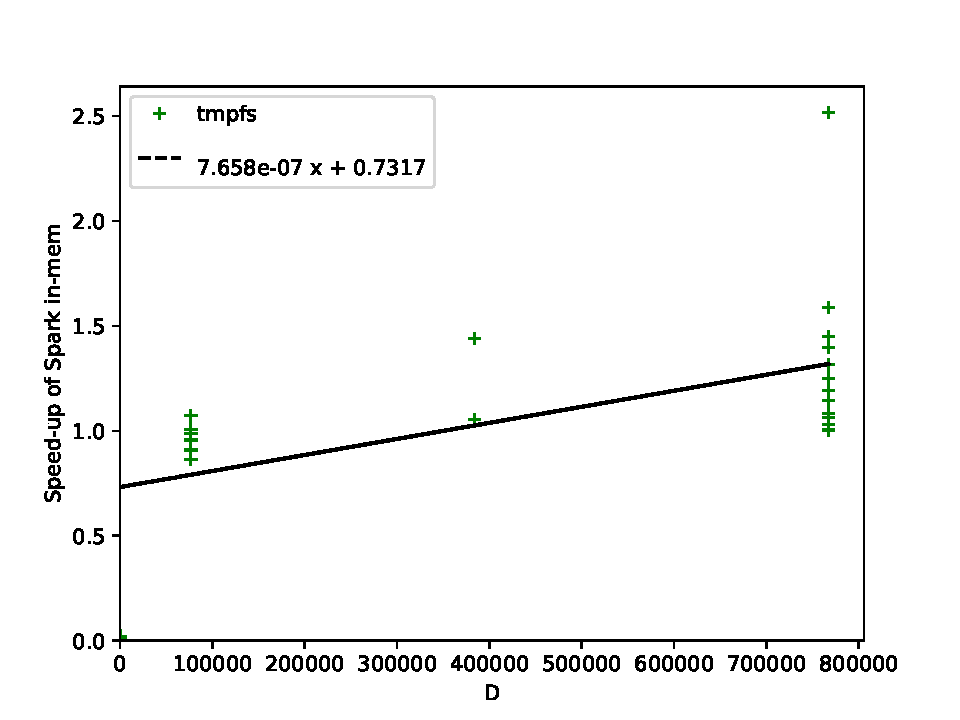
\includegraphics[width=\textwidth]{results/figures/tmpfs-incrementation.pdf}
\caption{}
\label{fig:sub1}
\end{subfigure}%
    \begin{subfigure}{0.33\linewidth}
\centering
    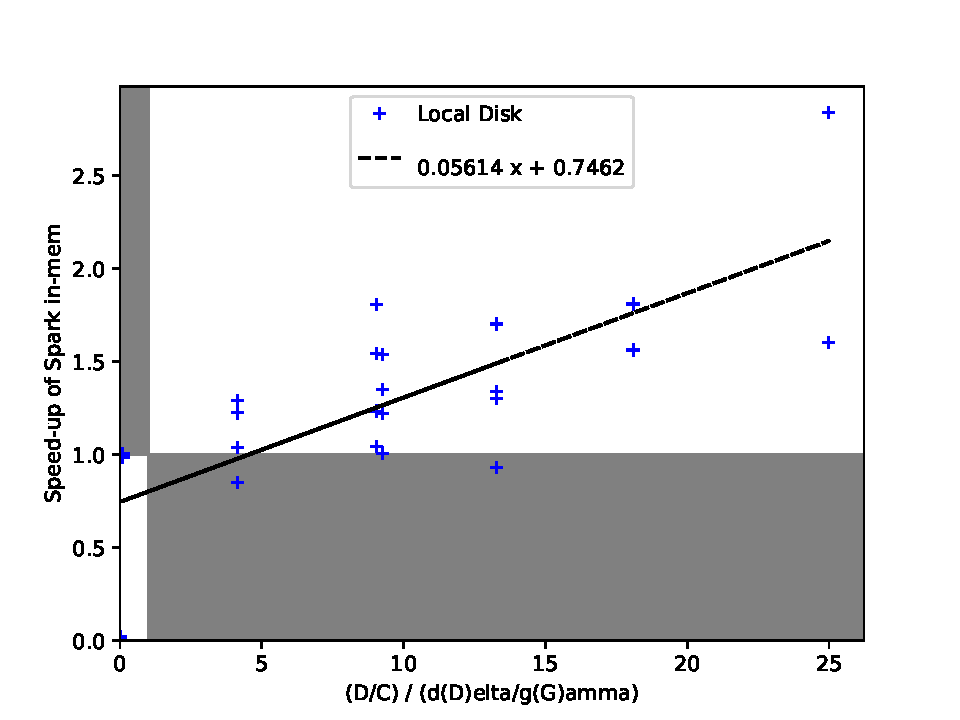
\includegraphics[width=\textwidth]{results/figures/local-incrementation.pdf}
\caption{}
\label{fig:sub2}
    \end{subfigure}%
\begin{subfigure}{0.33\linewidth}
\centering
    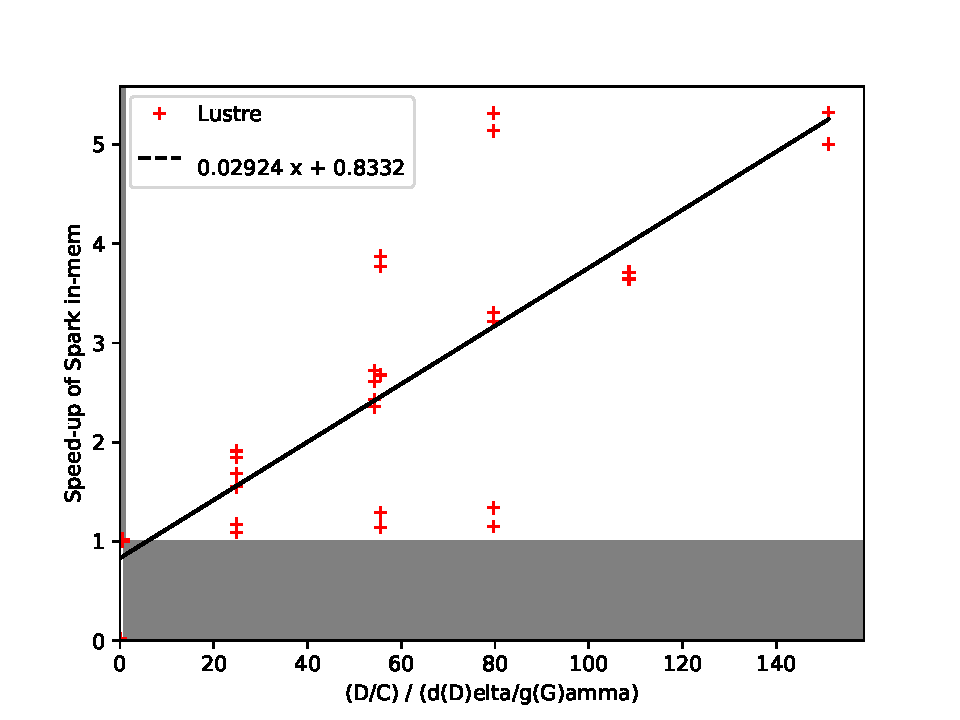
\includegraphics[width=\textwidth]{results/figures/lustre-incrementation.pdf}
\caption{}
\label{fig:sub3}
\end{subfigure}
    \caption{Model evaluation on (a) tmpfs, (b) local and (c) Lustre. Grey 
             regions denote areas that violate model predictions.}
\label{fig:modeleval}
\end{figure*}


% Incrementation (avoid cache effects in binarization)
In order to investigate how the different strategies impact processing, we 
selected a simple incrementation pipeline (Algorithm~\ref{alg:incrementation}) 
that consisted exclusively of map 
stages. A series of map-only stages would enable us to evaluate the effects of
in-memory computing when data locality is preserved. Incrementation was 
selected 
over other applications, such as binarization, as it ensured that a new image
was created at each step (i.e. no caching effects within the executing 
application). Each partitioned chunk was incremented by 1, in parallel, by
the processing engines. As incrementing the images is a relatively quick 
process, we added a sleep delay to the incrementation stage in order to 
increase task duration. The incremented chunks would be either 
maintained in-memory (Spark only) or saved to either tmpfs, local disk or 
Lustre (Spark and Nipype). Should more than a single iteration be requested, 
the increment chunks would be incremented again and saved to the same storage. 
This would repeat until the number of requested iterations had elapsed. In all 
conditions, the first input chunks would be reads from Lustre and the final 
output chunks would be saved to Lustre. We chose to perform our initial 
reads and final writes on Lustre as a multi-tenant clusters' compute node's 
local storage, if 
available, is generally temporary and only available for the duration of the 
allocation. 

\subsubsection{Setup}

For our first incrementation experiment, we investigated the effects of
in-memory computing on varying total data size. To do this, we increased the 
number of incrementation iterations from 1, 10 and 100 times. The total data 
size would then increase from 75GB, at 1 iteration, to 7500GB, at 100 
iterations. In order
to validate the model, the D/C was varied to fall in different regions of 
Equation~\ref{eq:page-cache-inequality}. The D/C selected were 256, 178.6, 80 
and 1.9MB/s\todo{present this as a table? yes, I think it would be clearer (TG) but not mandatory.}. 80 and 1.9MB/s satisfied the 
inequality for local disk, whereas only 1.9MB/s satisfied the inequality for 
Lustre. These D/C ratios were applied to each iteration experiment, such that 
we were able to get both the effect of increasing the total amount of data, in 
addition to, increasing the task duration for a given data size.

We combined the first experiment with our second experiment such that we could 
evaluate the effects of in-memory computing on varying task duration. If the 
page cache has sufficient time to flush, it should be expected that using 
in-memory computing should have no increased speed-up over disk. We maintained 
the D/C ratios as those mentioned above, but rather than applying only one to
a different number of iterations, we applied all four D/C to all numbers of 
iterations. That is 1 iteration, 10 iterations and 100 iterations were all 
processed with using the aforementioned D/C ratios.

As a third incrementation experiment, we were interested in the effects of 
chunk size on in-memory computing. Naturally, greater chunk size signifies 
a decrease in parallelization, however, it also means an increase in sequential
I/O. For this experiment we incremented the 30, 125 and 750 chunk complete
BigBrain image. The amount of parallelization for 30 chunks was 2 cores/node, 
whereas it was 9 cores/node for 125 chunks and 25 cores/node for 750 chunks. 
While Spark attempted to load-balance the data, it used up only 25 of the 40 
cores for 750 chunks. In contrast, Nipype tried to use up as many cores as 
possible. To ensure both engines were processing the same amount of data 
concurrently, we fixed the amount of cores used to 25.
Unlike the previous experiment, the D/C ratio was kept static at 174.4MB/s, 
however, this ratio ensured that different regions of the inequality were 
reached depending on amount of parallelization. A ratio of 174.4 MB/s satified
the inequality for local disk at 30 chunks. All other ratios did not satisfy 
the inequality for Lustre and local disk. Unfortunately, 30 chunks could no be 
processed using in-memory Spark as its individual chunk size of 3GB exceeded 
the 2GB partition size limit imposed by Spark.

For our fourth and final incrementation experiment, we investigated the effects 
of the strategies on different image sizes. We selected the 75GB BigBrain, the
38GB half BigBrain and the 13M T1W MRI image for this experiment. The number of
chunks was fixed at 125. Similarly to the previous experiment, the total 
sequential compute time was fixed, however, due to varying size in total data 
processed, the D/C ratio varied. Once again, we ensured that the D/C ratio fell
in multiple different regions of the inequality. The D/C ratio ranged from 
348.8 MB/s for BigBrain and 174.4MB/s for half Bigbrain, to 0.1MB/s for the MRI 
image. Only the 0.1MB/s MRI satisfied the inequality for both Lustre and local 
disk.

Since data-locality is not normally preserved in Nipype (a new SLURM allocation 
is requested for each processed task), we instrumented Nipype to ensure data 
locality. That is, for each chunk partition, we requested a SLURM allocation to
process the entire pipeline in parallel, using Nipype's MultiProc scheduler, on 
a given node. This was possible as no communication was required between the 
processed chunks.



% average (1 shuffle)
% Nipype: can't use SLURM plugin so had to actively poll.

% kmeans (many shuffles)

% Example BIDS app

% fmriprep?

% Explain how we tweaked scheduling in Nipype to make it similar to Spark, 
% otherwise we're only measuring scheduling differences. Needs a discussion on scheduling somewhere.

% Talk about our I/O pattern: random I/O, sequential.


\subsubsection{Execution modes} % perhaps find a better title, it's not informative

We tuned job scheduling to balance the load among
cluster nodes. This is the default behavior of Spark, but required
specific instrumentation in Nipype.


\section{Results} % 2 pages
\label{sec:results}

% We checked that scheduling was similar in both cases (show a two Gantt charts to illustrate)

\subsection{Model Evaluations}

In order to evaluate our model, we compared the observed in-memory speedup 
ratio to our model's expected speed-up ratio for the given 
D/C / $\delta$/$\gamma$ used (Figure~\ref{fig:modeleval}). Experiments for 
which there was no in-memory equivalent (i.e. BigBrain split into 30 chunks) 
were not considered.

%probably confusing to mention values, but they're here for now
Results show that, overall, the model correctly predicted the effect of page 
cache on processing times for local disk and Lustre. Points which violated 
model predictions were found at 1 iteration, where page cache would not have 
been saturated, due to the amount of data being written, and at a task duration
of 320 seconds. However, in all cases, the ``1" boundary was never trespassed by 
more than a factor of 0.19, and is therefore likely a result of system 
variability.

Lustre's regression slope is smallest of the three filesystems, possibly 
lending to the fact that Lustre was nearly always in transient state. Out of 
the thirty four benchmarks taken on Lustre, Lustre was only expected to be in steady 
state for four of the benchmarks (MRI and all benchmarks with a steady state of
320). This was validated by our experiments.

The next smallest slope is that of the local disk. The local disk was \todo{continue after disk benchmarks}

Unlike local disk and Lustre, tmpfs exists within the page cache and should not 
be affected by it in the same way. However, when memory is low, tmpfs will 
begin to write to the swap space, located on disk. As a result, it is possible 
to see similar trends to local disk when space is low. 
Figure~\ref{fig:modeleval} (a) shows that the speed-up between in-memory 
computing and tmpfs increases as the D/C / $\delta$/$\gamma$ ratio increases. 
This is unexpected as both tmpfs and in-mem reside in memory and should 
therefore both have comparable makespans. This was found to occur when the 
contention to RAM was highest. In other words, when 750 chunks were written to
disk in 10 iterations with a task duration of 0.59s, Spark in-memory was 
approximately 2x faster. 
%why is this? will generate gantts to investigate further.


\subsection{Iterations}
\begin{figure}[h]
    \centering
    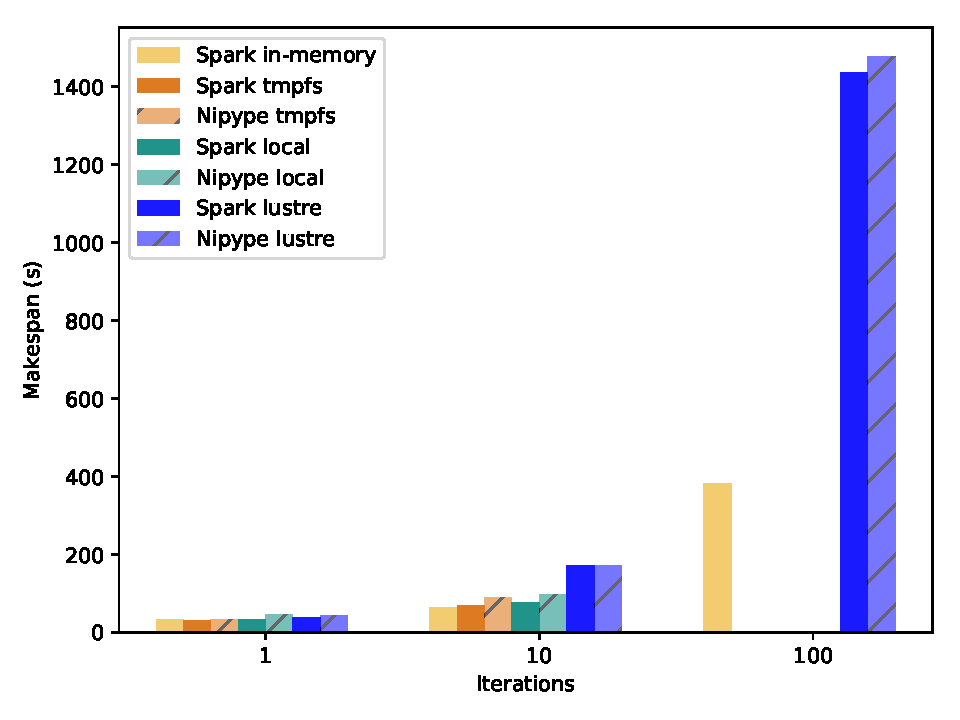
\includegraphics[width=\linewidth]{results/figures/iterations.pdf}
    \caption{Makespans of Spark and Nipype writing to memory, tmpfs, local 
             disk and Lustre for a given number of iterations. All 
             makespans use 125 chunks of the complete BigBrain and have a fixed
             task duration of 3.44 seconds}\label{fig:iterations}
\end{figure}


Figure~\ref{fig:iterations} shows the difference between the different 
filesystem choices given the number of iterations. At 1 iteration, all 
filesystems behave the same, as they are all writing to the page cache. As the 
total amount of data written by the application increases to 750~GB, there is a 
greater disparity between Lustre and in-memory (2.67~x slower, on average). 
Local disk performance, however, 
is still comparable to memory (1.38~x slower, on average). Despite local disk and 
Lustre both being in transient state, local disk encounters less contention 
than what would be found on Lustre. 

%sp_mem 1it = 34s, 10it = 64 100it = 381
%3.44 * 1 = 3.44, 3.44*10 = 34, 3.44*100 = 344

%sp_tmpfs 1it = 31, 10it = 69, 

At 100 iterations, or 7500~GB, Lustre can be found to be, on average, 3.82x 
slower than Spark in-memory. The page cache, on Zenith, occupies 20\% of 
available memory. Assuming all memory (187~GB) was available, only 37.4~GB of 
data could be held in a node's page cache at any given time. The slowdown 
experienced can be explained by the much less data could reside in the page 
cache at a given time, in contrast to 10 iterations, and therefore the effects 
of disk bandwidth are more significant in this workflow

While there is some variability that can be seen in Figure~\ref{fig:iterations} 
between the two engines, this believed to be insignificant, and potentially due 
to SLURM node allocation delays in our launching of Nipype.

% Comment on the general trend
% note 'on average' = average between spark and nipype. local disk spark is 
% 1.22x slower and local disk nipype is 1.54x slower
% spark lustre 2.66x slower; nipype lustre 2.68x slower

\subsection{CPU Time}
% Comment on the general trend
% We can't really say that imaging tasks are not small. Even Freesurfer could be decomposed.
%
\begin{figure}[h]
    \centering
    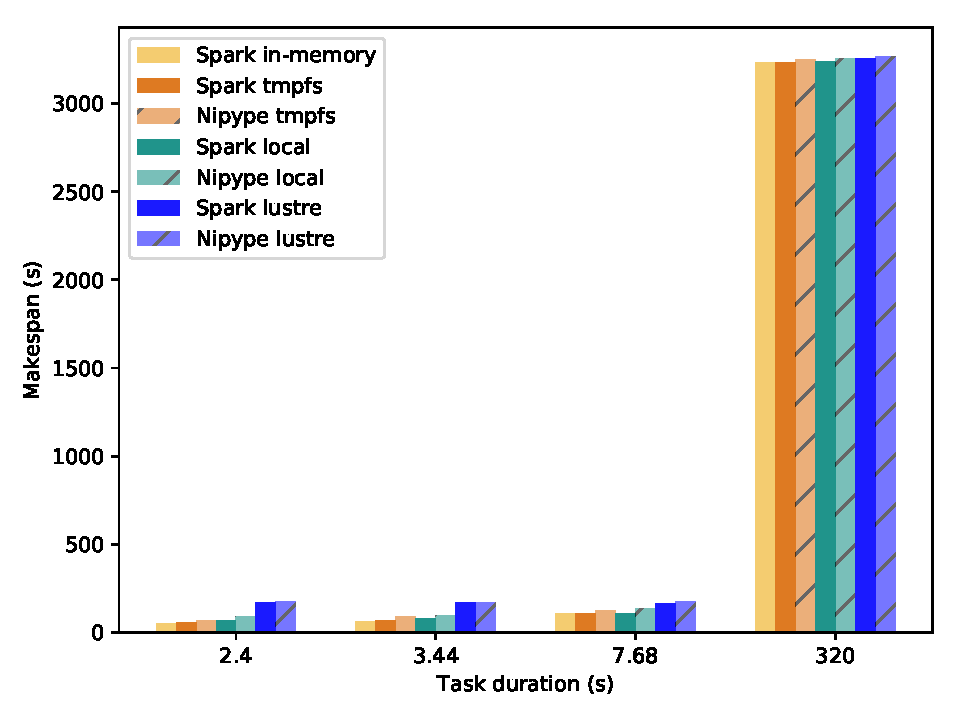
\includegraphics[width=\linewidth]{results/figures/cputime.pdf}
    \caption{Makespans of Spark and Nipype writing to memory, tmpfs, local 
             disk and Lustre with varying task durations. All 
             makespans use 125 chunks of the complete BigBrain and are fixed at 
             10 iterations}\label{fig:cputime}
\end{figure}

Increasing CPU time ensured that all filesystems had a comparable performance
(Figure~\ref{fig:cputime}). Lustre, for instance, is approximately 1.01x slower
than Spark in-memory at a task duration of 320 seconds, whereas it is 
approximately 3.25x slower that Spark in-memory with 2.4 second tasks. This 
pattern corroborated by our model which postulates that 
data movement costs will have little impact on compute-intensive tasks. The 
reasoning for this is that longer tasks give the page cache more time to flush 
between write to disk. The longer the delay, the less likely the page cache is 
to fill up when the concurrent data size written fits within the page cache.






\subsection{Image Block size}
\begin{figure}[h]
    \centering
    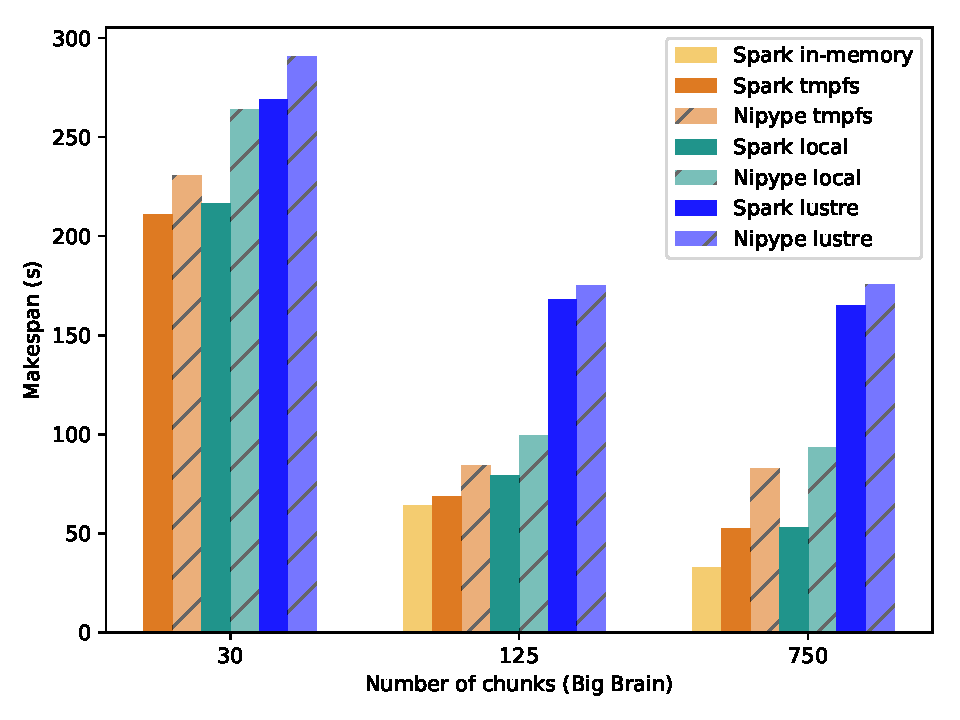
\includegraphics[width=\linewidth]{results/figures/numchunks.pdf}
    \caption{Makespans of Spark and Nipype writing to memory, tmpfs, local 
             disk and Lustre with varying numbers of chunks. All 
             makespans have the same overall sequential CPU time and 
             are fixed at 
             10 iterations}\label{fig:numchunks}
\end{figure}
% Comment on the general trend
As can be seen in Figure~\ref{fig:numchunks}, makespan decreases when the number 
of chunks increase. This is due to the fact that parallelism increases. With 
30 chunks, only 2 CPUs per node are actively working. At 125 chunks, this 
changes to a maximum of 9 CPUs per node, and at 750 chunks all 40 CPUs can be 
active. It can be noted that no significant speedup can be seen between 125 
chunks and 750 chunks. This is because out of the 50 chunks processed by each 
node, only 40 can be processed concurrently, thus requiring two sequential 
incrementation batches, and resulting in similar makespans as 125 
chunks.

In terms of filesystem selection, local and tmpfs perform comparably for all 
conditions, with Lustre being significantly slower. As with varying the number 
of iterations, Lustre is slower due to increased filesystem contention, which 
is, at minimum, 15x greater than contention on local disk. With an increase in 
number of chunks, local disk and tmpfs makespans begin to converge. A potential 
explanation for this may be that tmpfs is utilizing swap space. As concurrency 
increases, the memory footprint of the application also increases. It is 
possible that at 750 chunks, swapping to disk is required by tmpfs, thus 
resulting in similar processing times as local disk.

Swapping may also be an explanation for the variance between Spark in-memory 
and tmpfs performance. While Spark may also spill to disk, it only does so when
data does not fit in memory. As none of the RDDs generated throughout the 
pipeline were cached and all data concurrently accessed could be mantained 
in-memory, even for the 750 chunks which were processed in two batches, it did 
not need to spill to disk.

\subsection{Data Size}
\begin{figure}[h]
    \centering
    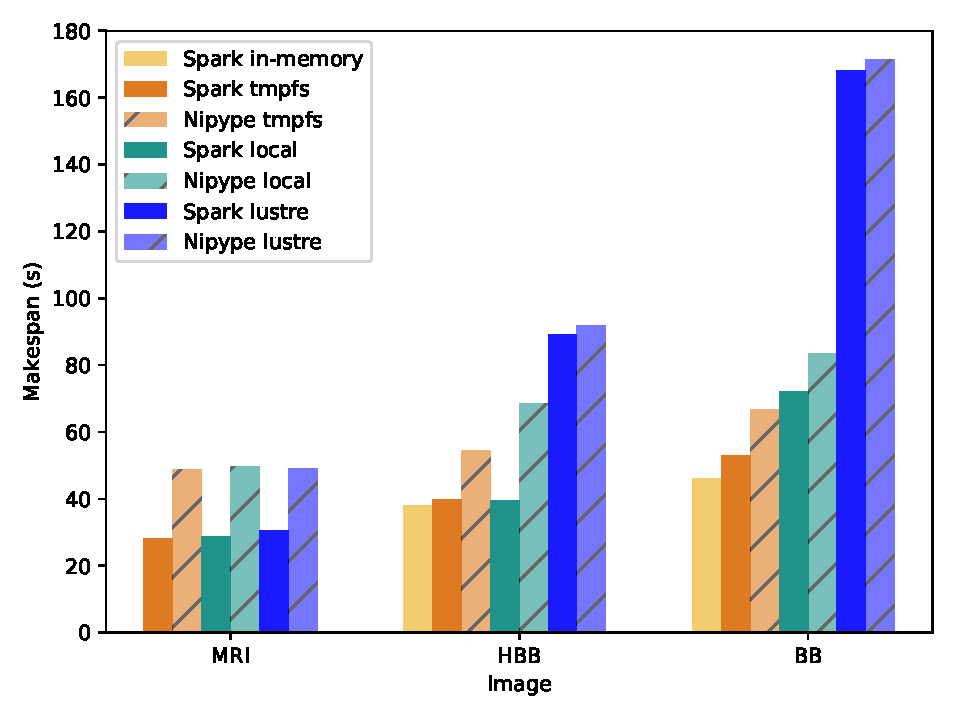
\includegraphics[width=\linewidth]{results/figures/datasize.pdf}
    \caption{Makespans of Spark and Nipype writing to memory, tmpfs, local 
             disk and Lustre with varying data sizes. All 
             makespans use 125 chunks and are fixed at 
             10 iterations with a task duration of 1.76 
             seconds }\label{fig:datasize}
\end{figure}
% Comment on the general trend
Increasing overall data size decreases performance, as can be seen in 
Figure~\ref{fig:datasize}. When the data size is very small, as is the case 
with the MRI image, all filesystem makespans are comparable. This is due to the 
fact that page cache can be leveraged fully regardless of file system. However, 
this time, Spark in-memory performed significantly worse than all other 
filesystems. Upon further inspection, it appeared that Spark in-memory executed
in a sequential order, on a single worker node. Lack of parallelism for the MRI 
image may be a result of Spark's max partition size, which is by default 128~MB
-- significantly larger than the 13~MB MRI image. Due to Spark in-memory's 
sequential execution, it was omitted from the graph.

At half BigBrain, the makespan differences become apparent in both local disk 
and Lustre, with Lustre, with Lustre becoming 2.4x slower than in-memory. This 
can be attributed to page cache saturation, as predicted by the model for both 
half the BigBrain image and the complete BigBrain. Only the MRI image was 
predicted to fall within the model constraints. 

When the complete BigBrain is processed, the disparity between the different 
filesystems becomes even greater. Lustre becomes 3.68x slower, whereas local 
disk is now 1.68x slower. The reasoning for this is that the page cache fills 
up faster than with half of BigBrain.

\todo{change Spark's max partition size and test to see if it fixes the problem}

% Interactive gantt charts?

\section{Discussion} % 2 pages
\label{sec:discussion}
\subsection{Effect of In-Memory Computing}
% Shared fs vs local disk vs in-memory: what do we gain?

\subsection{Effect of Data Locality}
% It should be important, in particular when there is contention and when
% tasks are small. 

% Effect of Lazy Evaluation?

\subsection{Can tmpfs and Page Caches Emulate In-Memory Computing?}
% tmpfs and local disks fill up: need cleanup.
% Can we emulate in-memory computing using write buffers or tmpfs?


\subsection{Scheduling Remarks}
% Scheduling: load balance as much as you can.
% (which isn't what nipype multiproc does)


A common recommendation in Spark is to limit the number of cores per 
executors to 5, to preserve a good I/O 
throughput\footnote{\url{http://blog.cloudera.com/blog/2015/03/how-to-tune-your-apache-spark-jobs-part-2}}. 
We believe that throughput degradation observed with more than 5 cores 
per executor might be coming from full page caches.

\subsection{Other Comments}

% fault-tolerance: if you loose a node, you loose the data when it's written on disk or in memory.
%                  then the only solution is to recompute, which spark would do automatically.
%                  when nipype is run on lustre, it would avoid recomputing existing files, which Spark doesn't do.
%                   this niype feature is lost when not using lustre.

% Comment on the practical implications of using tmpfs or local disk: we might not get all the intermediary files.

% mention burst buffers or heterogeneous storage managers as potential solutions to write to local disk, 
% i.e., to benefit from data locality while getting your results on Lustre. 

\subsection{Engine-Specific Comparisons}

% Spark vs Nipype
% Do we see the effect of Java serialization?

\section{Conclusion} % 1 page with refs
\label{sec:conclusion}
% When is it useful to use a Big Data engine?

% "```Disk and network I/O, of course, play a part in Spark performance 
% as well, but neither Spark nor YARN currently do anything to actively 
% manage them.```"
% http://blog.cloudera.com/blog/2015/03/how-to-tune-your-apache-spark-jobs-part-2/


% Future work:
% - scheduling in a shared environment.
% - workflow-aware cache eviction strategies instead of LRU/n

\section{Acknowledgments}

\todo{Acknowledge Dell and ask them if they want to co-author the paper.}

\bibliographystyle{IEEEtran} 
\bibliography{biblio}

\end{document}























